\documentclass{beamer}
\setbeamertemplate{navigation symbols}{}

\title{Seri}
\subtitle{A High-Level User Language for SMT Queries}
\author{Richard Uhler}

\begin{document}

\begin{frame}
    \titlepage
\end{frame}

\begin{frame}{Sudoku in Seri}
\begin{overprint}
\onslide<1> 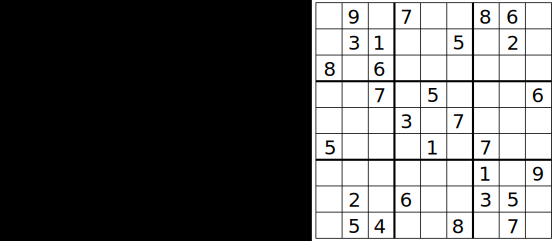
\includegraphics[width=\textwidth]{input1}
\onslide<2> 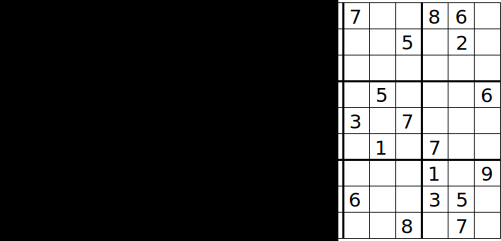
\includegraphics[width=\textwidth]{input2}
\end{overprint}
\end{frame}
 
\begin{frame}{Representing and Reading the Board}
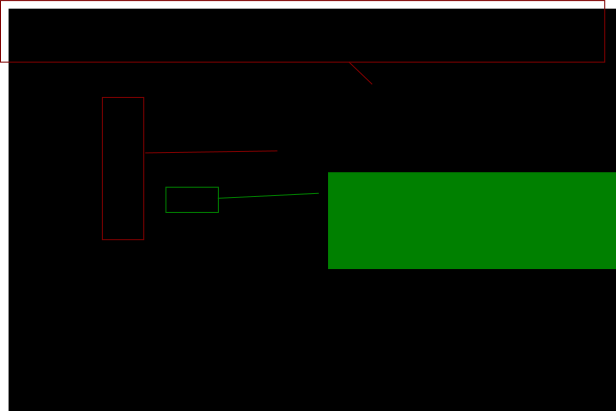
\includegraphics[width=\textwidth]{parser}
\end{frame}

\begin{frame}{The Sudoku Constraints}

\includegraphics[width=\textwidth]{isvalid}
\end{frame}

\begin{frame}{The Sudoku Solver}

\includegraphics[width=\textwidth]{main}
\begin{itemize}
\item Yices1: 1m15s
\item Yices2: 1.6s
\end{itemize}
\end{frame}

\begin{frame}{A Different Cell Representation}

\includegraphics[width=\textwidth]{bitcell}
\begin{itemize}
\item Yices1: 3m53s
\item Yices2: 1.0s
\end{itemize}
\end{frame}

\begin{frame}{Interactive Queries}

\includegraphics[width=\textwidth]{allq}
\end{frame}

\begin{frame}{Leveraging Different SMT Solvers}
\begin{block}{Our queries are independent of the SMT solver used}
Yices1 and Yices2 currently supported.
\end{block}
\begin{block}{Future Goals}
    \begin{itemize}
        \item Leverage the strength of specific solvers.
        \begin{itemize}
            \item datatypes directly (yices1)
            \item datatypes on top of tuples (yices2)
            \item datatypes on top of bit vectors
            \item datatypes on top of ???
        \end{itemize}

        \item Run query on array of solvers simultaneously.
    \end{itemize}
\end{block}
\end{frame}

\begin{frame}{Current Status, Future Work}
\begin{block}{Current Status}
    \begin{itemize}
        \item Yices1, Yices2 supported
        \item All queries shown work
    \end{itemize}
\end{block}
\begin{block}{Future Work (Ph.D. Thesis)}
    \begin{itemize}
        \item Improve performance of elaborator
        \item Add support for more solvers
        \item Take advantage of specific features in the different solvers
        \item Integrate tool seamlessly with haskell
        \item Explore implementation of formal tools such as model checkers
              built in Seri out of reusable library components
    \end{itemize}
\end{block}
\end{frame}

\end{document}

